\section{Résultats}

Comme mentionné en introduction, nous avons testé trois méthodes de vectorisation : TF-IDF, doc2vec et BERT
Nous avons utilisé ces vecteurs pour entraîner et comparer 4 modèles différents : Régression logistique, SVM, Random Forest et Perceptron.


\begin{table}[h]
    \centering
    \begin{tabular}{|l|l|l|l|l|}
        \hline
        Clf & RandomForest & SVM & Perceptron & LR \\
        \hline
        Anglais & 0.37 & \textbf{0.47} & 0.41 & 0.46 \\
        \hline
        Français & 0.34 & \textbf{0.45} & 0.42 & 0.44 \\
        \hline
        Italien & 0.33 & \textbf{0.43} & 0.40 & 0.43 \\
        \hline
    \end{tabular}
    \caption{F-mesure des classifieurs par langue avec vectorisation \texttt{TF-IDF}}
    \label{tab:comparaison_vecteurs}
\end{table}

\begin{table}[h]
    \centering
    \begin{tabular}{|l|l|l|l|l|}
        \hline
        Clf & RandomForest & SVM & Perceptron & LR \\
        \hline
        Anglais & 0.29 & \textbf{0.39} & 0.22 & 0.31 \\
        \hline
        Français & 0.26 & \textbf{0.34} & 0.25 & 0.28 \\
        \hline
        Italien & 0.27 & \textbf{0.33} & 0.22 & 0.28 \\
        \hline
    \end{tabular}
    \caption{F-mesure des classifieurs par langue avec vectorisation \texttt{Doc2Vec}}
    \label{tab:comparaison_vecteurs}
\end{table}

\begin{table}[h]
    \centering
    \begin{tabular}{|l|l|l|l|l|}
        \hline
        Clf & RandomForest & SVM & Perceptron & LR \\
        \hline
        Anglais & 0.32 & \textbf{0.32} & 0.22 & 0.36 \\
        \hline
        Français & 0.31 & \textbf{0.27} & 0.13 & 0.36 \\
        \hline
        Italien & 0.31 & \textbf{0.26} & 0.15 & 0.36 \\
        \hline
    \end{tabular}
    \caption{F-mesure des classifieurs par langue avec vectorisation \texttt{BERT}}
    \label{tab:comparaison_vecteurs}
\end{table}

\begin{figure}[t]
  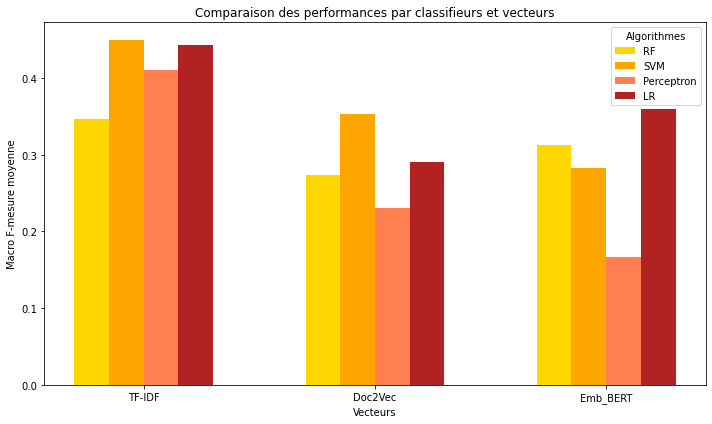
\includegraphics[width=\columnwidth]{"./assets/comparaison_vecteur_clf_barplot.png"}
  \caption{Comparaison des vecteurs et classifieurs.}
  \label{fig:comparaison_vecteur}
\end{figure}

\par En ce qui concerne les vecteurs, les meilleurs résultats observés ont été obtenus à partir de \texttt{TF-IDF} : le meilleur classifieur a une f-mesure de 0.47 avec ces vecteurs, tandis que le meilleur à partir de \texttt{Doc2Vec} est à 0.39 et à partir de \texttt{BERT} 0.36. De façon générale, les résultats ont tendance à être supérieurs avec cette méthode de vectorisation. Bien que \texttt{BERT} et \texttt{Doc2Vec} démontrent des performances similaires, cette dernière méthode est celle qui performe le mieux des deux.
\par Globalement, les résultats sont relativement homogènes entre les langues. Avec le \texttt{TF-IDF}, la moyenne sur l'anglais de tous les modèles est à 0.47, 0.44 pour le français et 0.43 pour l'italien. Celui qui performe le moins est le Random Forest (f-mesure moyenne 0.32 sur l'anglais). 
\par Au niveau des classifieurs, on constate relativement peu de disparités entre leurs performances également. De manière générale, le meilleur classifieur est le SVM (en moyenne à 0.39 sur l'anglais en combinant toutes les méthodes de vectorisation), toutefois relativement proche de la Régression logistique (f-mesure moyenne à  0.37).